\documentclass[t]{beamer}
\usetheme{Copenhagen}
\setbeamertemplate{headline}{} % remove toc from headers
\beamertemplatenavigationsymbolsempty

\usepackage{amsmath, array, tikz, bm, pgfplots, tcolorbox, graphicx, venndiagram, color, colortbl}
\pgfplotsset{compat = 1.16}
\usepgfplotslibrary{statistics}
\usetikzlibrary{calc}

\title{Qualitative Graphs}
\author{}
\date{}

\AtBeginSection[]
{
  \begin{frame}
    \frametitle{Objectives}
    \tableofcontents[currentsection]
  \end{frame}
}

\begin{document}

\begin{frame} 
\maketitle
\end{frame}

\begin{frame}{Why Bother with a Graph?}
With all of the tools and techniques available for working with data, why should we bother to obtain a visualizaiton of it?	\newline\\	\pause

Can provide you with all of the data regarding a car: make, model, color, mileage, maintenance and repair history, etc. but ultimately...	\pause
\begin{center}
\color{blue}\textbf{You would want to know at least know what it looks like.}
\end{center}
\vspace{10pt}	\pause
The same principal can be applied to datasets.
\end{frame}

\section{Create and interpret bar graphs}

\begin{frame}{Bar Graphs}
\begin{tcolorbox}[colframe=green!20!black, colback = green!30!white,title=\textbf{Bar Graph}]
A \textbf{bar graph} is a visual display of data in which bars are plotted, where one dimension represents each category and the other dimension represents the frequency (or relative frequency) of each category.
\end{tcolorbox}
\vspace{6pt}	\pause
\begin{center}
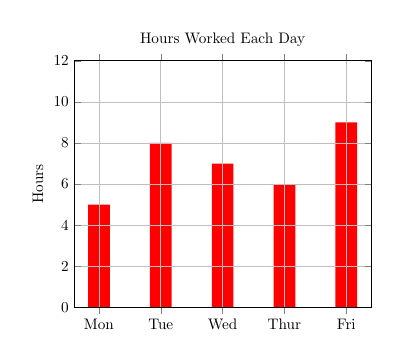
\begin{tikzpicture}[scale=0.55]
\begin{axis}[
ybar, axis on top, title={Hours Worked Each Day}, bar width = 0.5cm, grid,
ymin = 0, ymax = 12, ylabel = {Hours},
symbolic x coords = {Mon, Tue, Wed, Thur, Fri}, xtick=data
]
\addplot [draw=none, fill=red] coordinates{
	(Mon,5) (Tue,8) (Wed,7) (Thur,6) (Fri,9)
};
\end{axis}
\end{tikzpicture}
\end{center}
\end{frame}

\begin{frame}{Bar Graphs}
Bar graphs can be clustered:	\newline\\
\begin{center}
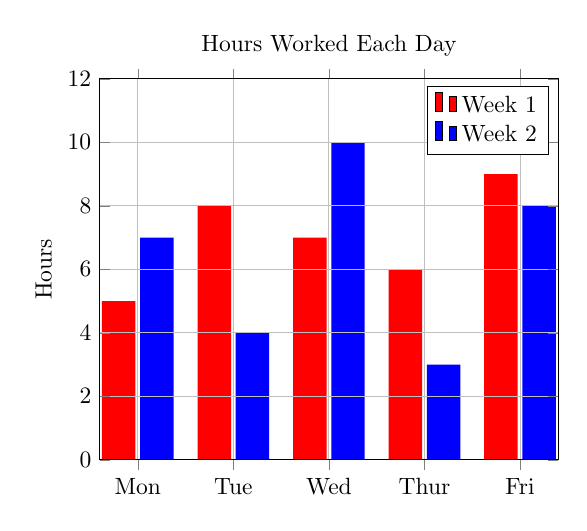
\begin{tikzpicture}[scale=0.85]
\begin{axis}[
ybar, axis on top, title={Hours Worked Each Day}, bar width = 0.5cm, grid,
ymin = 0, ymax = 12, ylabel = {Hours}, legend entries = {Week 1, Week 2},
symbolic x coords = {Mon, Tue, Wed, Thur, Fri}, xtick=data
]
\addplot [draw=none, fill=red] coordinates{
	(Mon,5) (Tue,8) (Wed,7) (Thur,6) (Fri,9)
};
\addplot [draw=none, fill=blue] coordinates{
	(Mon,7) (Tue,4) (Wed,10) (Thur,3) (Fri,8)
};
\end{axis}
\end{tikzpicture}
\end{center}
\end{frame}

\begin{frame}{Bar Graphs}
Bar graphs can be stacked:	\newline\\
\begin{center}
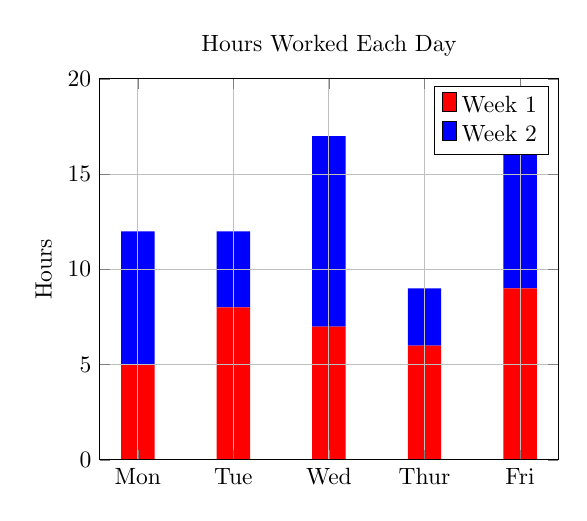
\begin{tikzpicture}[scale=0.85]
\begin{axis}[
ybar stacked, axis on top, title={Hours Worked Each Day}, bar width = 0.5cm, grid,
ymin = 0, ymax = 20, ylabel = {Hours}, legend entries = {Week 1, Week 2},
symbolic x coords = {Mon, Tue, Wed, Thur, Fri}, xtick=data
]
\addplot [draw=none, fill=red] coordinates{
	(Mon,5) (Tue,8) (Wed,7) (Thur,6) (Fri,9)
};
\addplot [draw=none, fill=blue] coordinates{
	(Mon,7) (Tue,4) (Wed,10) (Thur,3) (Fri,8)
};
\end{axis}
\end{tikzpicture}
\end{center}
\end{frame}

\begin{frame}{Bar Graphs}
Bar graphs can be horizontal:	\newline\\
\begin{center}
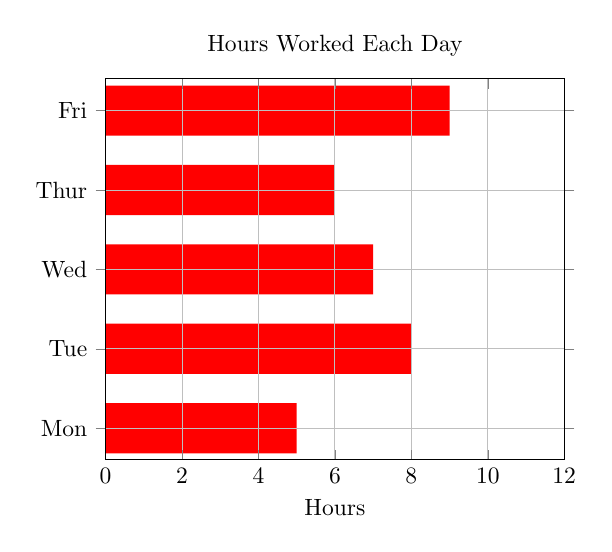
\begin{tikzpicture}[scale=0.85]
\begin{axis}[
xbar, axis on top, title={Hours Worked Each Day}, bar width = 0.75cm, grid,
xmin = 0, xmax = 12, xlabel = {Hours},
symbolic y coords = {Mon, Tue, Wed, Thur, Fri}, ytick=data
]
\addplot [draw=none, fill=red] coordinates{
	(5,Mon) (8,Tue) (7,Wed) (6,Thur) (9,Fri)
};
\end{axis}
\end{tikzpicture}
\end{center}
\end{frame}

\begin{frame}{Bar Graphs}
Bar graphs can show relative frequency (percent of total):	\newline\\
\begin{center}
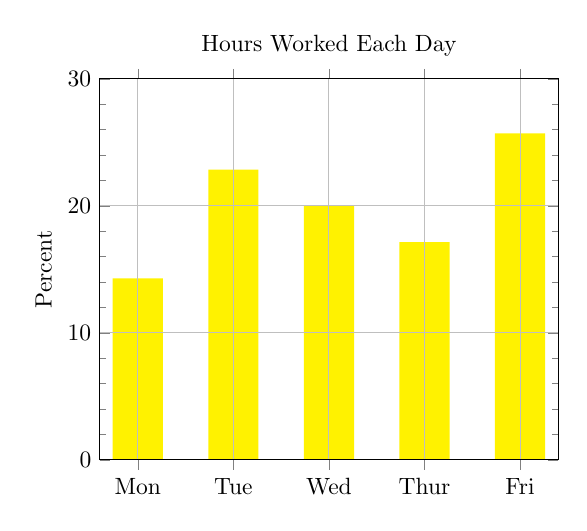
\begin{tikzpicture}[scale=0.85]
\begin{axis}[
ybar, axis on top, title={Hours Worked Each Day}, bar width = 0.75cm, grid,
ymin = 0, ymax = 30, ylabel = {Percent}, minor y tick num = 4,
symbolic x coords = {Mon, Tue, Wed, Thur, Fri}, xtick=data
]
\addplot [draw=none, fill=yellow] coordinates{
	(Mon,14.29) (Tue,22.86) (Wed,20) (Thur,17.14) (Fri,25.71)
};
\end{axis}
\end{tikzpicture}
\end{center}
\end{frame}

\begin{frame}{Creating a Bar Graph}
To create a bar graph, it helps to get a frequency chart of the information. \newline\\	\pause

A frequency chart displays the count of each observation, which can also be used to create a relative frequency chart.	\newline\\	\pause
\begin{center}
\begin{tabular}{c|c|c}
\textbf{Day} & \textbf{Hours Worked} & \textbf{Percent Total} \\ \hline
Monday 		& 	5	&	14.29\%	\\
Tuesday 	& 	8	&	22.86\%	\\
Wednesday	&	7	&	20.00\%	\\
Thursday	&	6	&	17.14\%	\\
Friday		&	9	&	25.71\%	\\
\end{tabular}
\end{center}
\end{frame}

\begin{frame}{Example 1}
One week, a questionnaire was given to hotel guests asking them to rate their satisfaction with their experiene. The ratings ranged from 1 (not satisfied) to 5 (very satisfied). Construct a bar graph of the data below:	\newline\\
\begin{center}
\begin{tabular}{cccccc}
2&3&1&2&3&4\\
1&5&5&2&2&4\\
5&3&2&5&3&4\\
4&3&5&1&1&1\\
3&5&3&1&4&5
\end{tabular}
\end{center}
\end{frame}

\begin{frame}{Example 1}
First, create a frequency distribution:	\newline\\	\pause
\begin{center}
\begin{tabular}{c|c}
\textbf{Rating} & \textbf{Frequency} \\ \hline
One & 6 \\
Two & 5 \\
Three & 7 \\
Four & 5 \\
Five & 7 
\end{tabular}
\end{center}
\end{frame}

\begin{frame}{Example 1}
\begin{center}
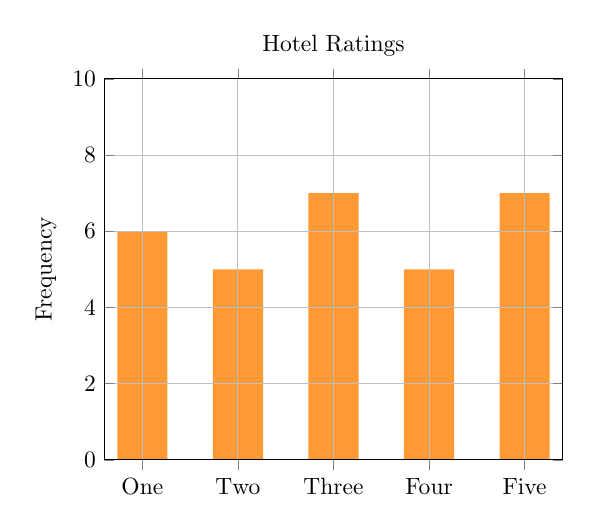
\begin{tikzpicture}[scale=0.85]
\begin{axis}[
ybar, axis on top, title={Hotel Ratings}, bar width = 0.75cm, grid,
ymin = 0, ymax = 10, ylabel = {Frequency},
symbolic x coords = {One, Two, Three, Four, Five}, xtick=data
]
\addplot [draw=none, fill=orange!80] coordinates{
	(One,6) (Two,5) (Three,7) (Four,5) (Five,7)
};
\end{axis}
\end{tikzpicture}
\end{center}
\end{frame}

\begin{frame}{Example 2}
Construct a relative frequency bar graph of the hotel ratings.	\newline\\	\pause
\begin{center}
\begin{tabular}{c|c|c}
\textbf{Rating} & \textbf{Frequency} & \textbf{Relative Frequency} \\ \hline
One & 6 & 1/5 \\
Two & 5 & 1/6\\
Three & 7 & 7/30 \\
Four & 5 & 1/6 \\
Five & 7 & 7/30 
\end{tabular}
\end{center}
\end{frame}

\begin{frame}{Example 2}
\begin{center}
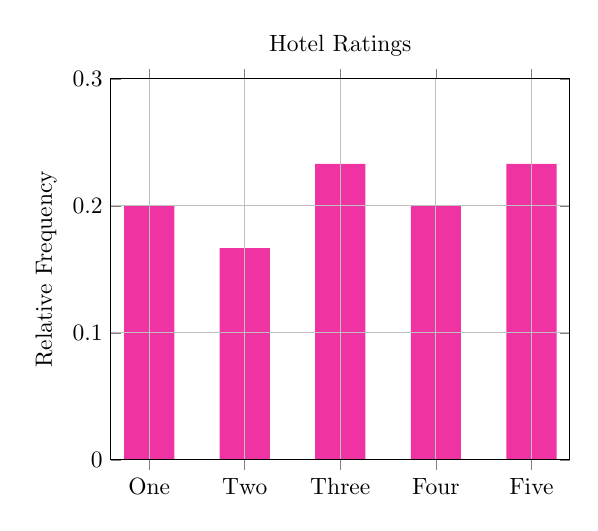
\begin{tikzpicture}[scale=0.85]
\begin{axis}[
ybar, axis on top, title={Hotel Ratings}, bar width = 0.75cm, grid,
ymin = 0, ymax = 0.3, ylabel = {Relative Frequency},
symbolic x coords = {One, Two, Three, Four, Five}, xtick=data
]
\addplot [draw=none, fill=magenta!80] coordinates{
	(One,0.2) (Two,0.1667) (Three,0.233) (Four,0.2) (Five,0.233)
};
\end{axis}
\end{tikzpicture}
\end{center}
\end{frame}

\begin{frame}{Example 3}
Seeing the results of the questionnaires, the hotel made some changes and the following month, asked 40 new guests to rate their experience. The results, along with the previous results are listed:	\newline\\
\begin{center}
\begin{tabular}{c|c|c}
\textbf{Rating} & \textbf{Frequency (Sample 1)} & \textbf{Frequency (Sample 2)} \\ \hline
One & 6 & 4 \\
Two & 5 & 3 \\
Three & 7 & 12 \\
Four & 5 & 10 \\
Five & 7 & 12 
\end{tabular}
\end{center}
Construct a stacked bar graph of the results.
\end{frame}

\begin{frame}{Example 3}
\begin{center}
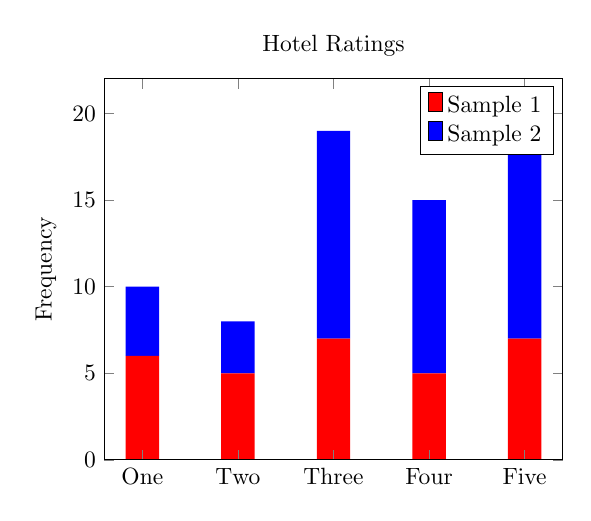
\begin{tikzpicture}[scale=0.85]
\begin{axis}[
ybar stacked, axis on top, title={Hotel Ratings}, bar width = 0.5cm, 
ymin = 0, ymax = 22, ylabel = {Frequency}, legend entries = {Sample 1, Sample 2},
symbolic x coords = {One, Two, Three, Four, Five}, xtick=data
]
\addplot [draw=none, fill=red] coordinates{
	(One,6) (Two,5) (Three,7) (Four,5) (Five,7)
};
\addplot [draw=none, fill=blue] coordinates{
	(One,4) (Two,3) (Three,12) (Four,10) (Five,12)
};
\end{axis}
\end{tikzpicture}
\end{center}
\end{frame}

\begin{frame}{Example 4}
Given the bar graph below, find the percent of people who travel in the summer.	\newline\\
\begin{minipage}{0.6\textwidth}
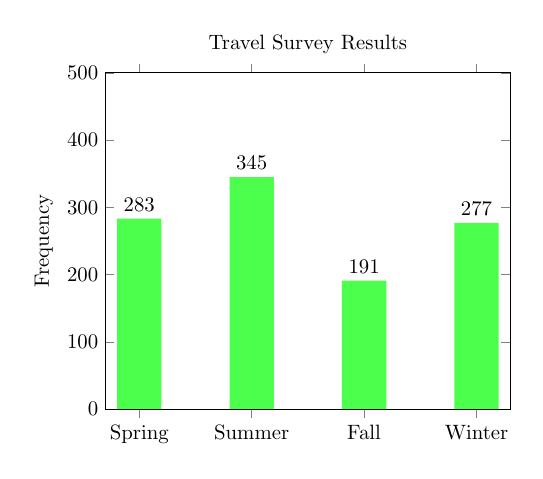
\begin{tikzpicture}[scale=0.75]
\begin{axis}[
ybar, axis on top, title={Travel Survey Results}, bar width = 0.75cm,
ymin = 0, ymax = 500, ylabel = {Frequency},
symbolic x coords = {Spring, Summer, Fall, Winter}, xtick=data, nodes near coords
]
\addplot [draw=none, fill=green!70] coordinates{
	(Spring,283) (Summer,345) (Fall,191) (Winter,277)
};
\end{axis}
\end{tikzpicture}
\end{minipage}
\hspace{10pt}
\begin{minipage}{0.3\textwidth}
\onslide<2->{Total: 1096} \\[10pt]
\onslide<3->{345/1096} \\[8pt]
\onslide<4->{$\approx$ 31.48\%}
\end{minipage}
\end{frame}

\begin{frame}{Pareto Charts}
\begin{tcolorbox}[colframe=green!20!black, colback = green!30!white,title=\textbf{Pareto Chart}]
A \textbf{Pareto chart} is a bar graph in which the data is listed in descending order of frequency or relative frequency.
\end{tcolorbox}
\vspace{6pt} \pause
\begin{center}
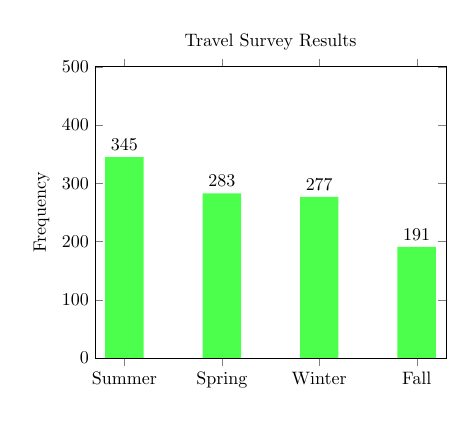
\begin{tikzpicture}[scale=0.65]
\begin{axis}[
ybar, axis on top, title={Travel Survey Results}, bar width = 0.75cm,
ymin = 0, ymax = 500, ylabel = {Frequency},
symbolic x coords = {Summer, Spring, Winter, Fall}, xtick=data, nodes near coords
]
\addplot [draw=none, fill=green!70] coordinates{
	 (Summer,345) (Spring,283) (Winter,277) (Fall,191) 
};
\end{axis}
\end{tikzpicture}
\end{center}
\end{frame}

\section{Interpret pie graphs}

\begin{frame}{Bar Graphs vs. Pie Graphs}
A good visual display of qualitative information, especially when dealing with relative frequency (percent), is the pie graph.	\newline\\	\pause

Pie graphs allow for quick comparison of the part-to-whole nature of percentage. \newline\\	\pause

Each slice of the pie (the central angle) is proportional to the percentage that slice is of the whole.
\end{frame}

\begin{frame}{Example 5}
The pie chart below represents the hours worked each day as a percentage of the week. What total percent of the week was spent working on Monday and Tuesday?	\newline\\
\begin{minipage}{0.5\textwidth}
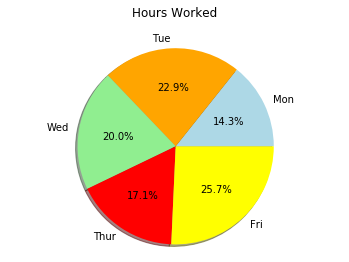
\includegraphics[scale=0.6]{../Images/pie.png}
\end{minipage}
\hspace{20pt}
\begin{minipage}{0.3\textwidth}
\onslide<2->{\[14.3\% + 22.9\%\]}	
\onslide<3->{ = 37.2\%}
\end{minipage}
\end{frame}



\end{document}